\documentclass[a4paper,10pt,oneside,final]{article}


\usepackage[english]{babel}
\usepackage[T1]{fontenc}
\usepackage{tabularx}
\usepackage[usenames,dvipsnames]{color}
\usepackage[table]{xcolor}
\usepackage[left=3.0cm, right=2.5cm, top=2.5cm, bottom=2.5cm]{geometry}
\usepackage{graphicx}
\usepackage{float}
\usepackage{caption}
\usepackage{listings}


\lstdefinestyle{ccc} 
{ 
numbers=none, 
basicstyle=\small\ttfamily, 
keywordstyle=\bf\color[rgb]{0,0,0}, 
%commentstyle=\color[rgb]{0.133,0.545,0.133}, 
stringstyle=\color[rgb]{0.627,0.126,0.941}, 
backgroundcolor=\color{white}, 
frame=tb, %frame= lrtb, 
framerule=0.5pt, 
linewidth=\textwidth,
%aboveskip=-4.0pt,
%belowskip=-4.0pt,
lineskip=-5.0pt,
}

%
% Define author(s) and  component's name
%
\def\defauthor{Lasse Lehtonen}
\def\deftitle{PKT\_CODEC\_MK2\\Reference Manual}



\author{\defauthor}
\title{\deftitle}

\usepackage{fancyhdr} 
\pagestyle{fancy} 
\lhead{\bfseries Department of Computer Systems\\
  Faculty of Computing and Electrical Engineering}
\chead{} 
\rhead{\bfseries \deftitle} 
\lfoot{\thepage} 
\cfoot{}
\rfoot{
\includegraphics[height=1.0cm]{pic/tty_logo.png}}
\renewcommand{\headrulewidth}{0.4pt}
\renewcommand{\footrulewidth}{0.4pt}


\def\deftablecolora{blue!10!white}
\def\deftablecolorb{white}

\begin{document}


%\maketitle
%\thispagestyle{empty}

\begin{titlepage}
\begin{center}

\vspace{6.0cm}
\textsc{\LARGE Tampere University of Technology}\\[1.0cm]
\textsc{\Large Faculty of Computing and Electrical Engineering}\\[1.0cm]
\textsc{\Large Department of Computer Systems}\\[1.0cm]
\vspace{6.0cm}
\hrule
\vspace{0.4cm}
{ \huge \bfseries PKT\_CODEC\_MK2\\\vspace{10pt}Reference Manual}
\vspace{0.4cm}
\hrule

%\vspace{2.0cm}

\vfill

\begin{minipage}{0.4\textwidth}
\begin{flushleft} \large
\emph{Author:}\\
\defauthor
\end{flushleft}
\end{minipage}
\begin{minipage}{0.4\textwidth}
\begin{flushright} \large
\emph{Updated:} \\
\today
\end{flushright}
\end{minipage}

\end{center}
\end{titlepage}

\newpage
\tableofcontents



\newpage
\section{REVISION HISTORY}
\setcounter{page}{1}

\begin{center}
  \rowcolors{3}{\deftablecolora}{\deftablecolorb}
  
  \captionof{table}{}
  \begin{tabularx}{\textwidth}{|lllX|}
    \hline
    Revision & Author          & Date       & Description\\
    \hline
    1.00  & Lasse Lehtonen  & 09.11.2011 & Initial documentation\\
    & & & \\
    & & & \\
    & & & \\
    & & & \\
    \hline
  \end{tabularx}
\end{center}



\newpage
\section{DOCUMENT OVERVIEW}

\subsection{SCOPE}

This documentation describes how to interface with NoCs using
pkt\_codec\_mk2 interface.

\subsection{AUDIENCE}

For hardware integrators wanting to use this component.

\subsection{RELATED DOCUMENTATION}

\begin{center}
  \rowcolors[]{2}{\deftablecolora}{\deftablecolorb}

  \captionof{table}{}
  \begin{tabularx}{\textwidth}{|lX|}
    \hline
    Document & Description\\
    \hline    
    & \\
    & \\
    & \\
    & \\
    \hline
  \end{tabularx}
\end{center}

\subsection{DOCUMENT CONVENTIONS}


\begin{itemize}
\item Ports: \texttt{teletype} in text
\item Generics: \texttt{teletype} in text
\end{itemize}



\newpage
\section{INTRODUCTION}

\subsection{BRIEF DESCRIPTION}

PKT\_CODEC\_MK2 is a network interface component placed between the IP
and the network. It handles the clock domain crossing and the
generation of the network depended packet headers. Supported
addressing modes include memory mapped, target id and raw where ip is
responsible for using correct network address.


%\subsection{EXAMPLE SYSTEM}


%\begin{center}  
%  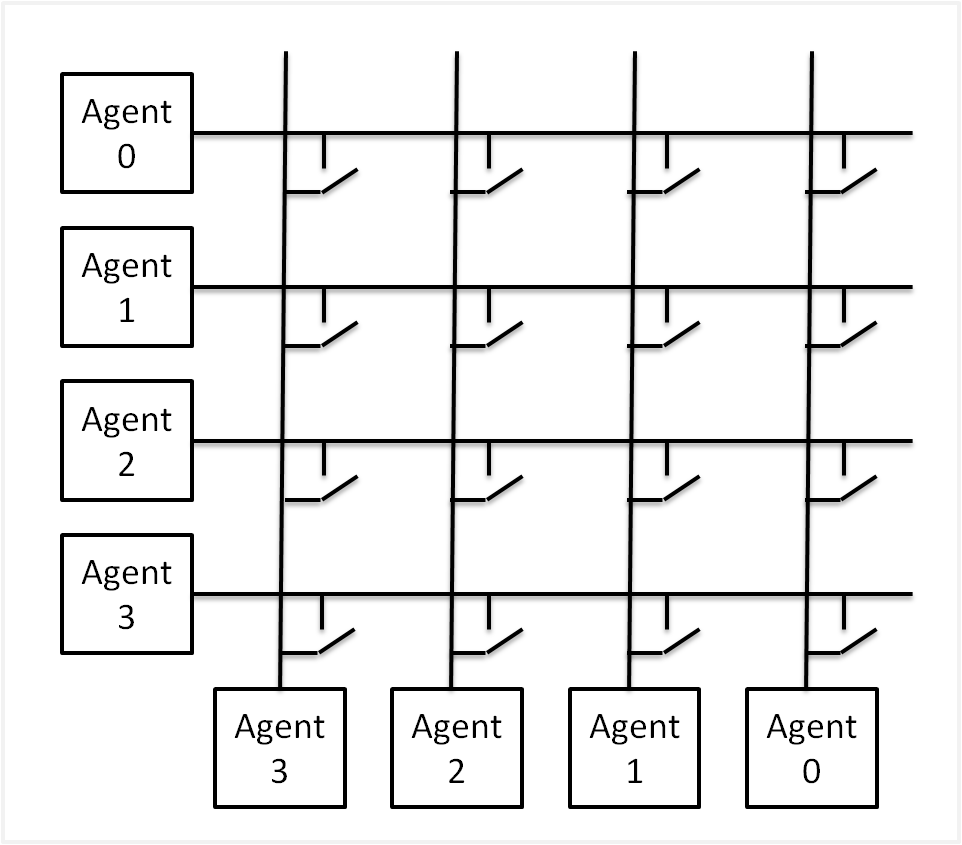
\includegraphics[width=0.8\textwidth]{pic/example_system.png}
%  \captionof{figure}{}  
%  \label{fig:example_system}
%\end{center}



\newpage
\section{HARDWARE DESIGN}

\subsection{PKT\_CODEC\_MK2}

\subsubsection{GENERICS}

\begin{center}
  \rowcolors{3}{\deftablecolora}{\deftablecolorb}

  \captionof{table}{}
  \begin{tabularx}{\textwidth}{|lX|}
    \hline
    Name                & Description\\
    \hline
    my\_id\_g           & Id number for addressing the agent\\
    cmd\_width\_g       & Width of the command bus\\
    data\_width\_g      & Width of the data bus\\
    agents\_g           & Total number of agents in the network\\
    cols\_g             & Columns in mesh like networks\\
    rows\_g             & Rows in mesh like networks\\
    agent\_ports\_g     & How many agents are connected to a router\\
    addr\_flit\_en\_g   & Transfer the original address with the packet\\
    address\_mode\_g    & Select addressing mode to use\\
    clock\_mode\_g      & Select asynchronous clock\\
    rip\_addr\_g        & Remove the network address from the packet\\
    noc\_type\_g        & Select the network model to use\\
    \hline
  \end{tabularx}
\end{center}

\subsubsection{CLOCKING AND RESET}

\begin{center}
  \rowcolors{3}{\deftablecolora}{\deftablecolorb}

  \captionof{table}{}
  \begin{tabularx}{\textwidth}{|lllX|}
    \hline
    Port   & Width & Direction & Description\\
    \hline
    clk\_net  & 1     & in      & Clock for the network, active on rising edge\\
    clk\_ip   & 1     & in      & Clock for the IP, active on rising edge\\
    rst\_n & 1     & in         & Reset, asynchronous, active low\\
    \hline
  \end{tabularx}
\end{center}

When \texttt{clock\_mode\_g} is 0 both clock inputs should be
connected to the same clock source and when 1 they can be connected to
asynchronous clocks.

\subsubsection{DATA INTERFACE}

\begin{center}
  \rowcolors{3}{\deftablecolora}{\deftablecolorb}

  \captionof{table}{}
  \begin{tabularx}{\textwidth}{|lllX|}
    \hline
    Port   & Width & Direction & Description\\
    \hline
    cmd\_in    & 2 & in  & Incoming command\\
    data\_in   & g & in  & Incoming data\\
    stall\_out & 1 & out & Stall the incoming data\\
    cmd\_out   & 2 & out & Outgoing command\\
    data\_out  & g & out & Outgoing data\\
    stall\_in  & 1 & in  & Stall sending data\\
    \hline
  \end{tabularx}
\end{center}

Zero on command line means that the line does not contain
anything. One means that on the data bus there's a address for the
next data flits. Two means there's data to be sent to the previous address.
Value three is undefined. Flow control is simple: at the clock cycle
when stall signal is read being high the corresponding command and
data lines must remain unmodified.

Format of the address depends on the \texttt{address\_mode\_g}
generic. Zero means that the IP should generate the network address
directly, one that address should be the id number of the target IP
and two that memory mapped addresses are used. Memory map translation
table can be defined in \texttt{addr\_lut.vhd}.




\end{document}
